\begin{solution}
The correct answer is $
(\binom{40 }{25} - \binom{40}{26}) \cdot 25! \cdot 15!$.\\[0.2cm]

Let $m$ be the number of people who have $5$ dollar bills and $n$ be the number of people who have $10$ dollar bills.
We show the configuration of a permutation of the people in the queue with a diagram similar to the one below, where we start from the origin and if the next person has $5$ dollar bills, we go to the top right, and if he only has $10$ dollar bills, we go to the bottom right.

In order to keep the diagram small, instead of $m=25$ and $n=15$ for the main problem,  we show an example diagram for  $m=6$ and $n=4$. 

\begin{center}
	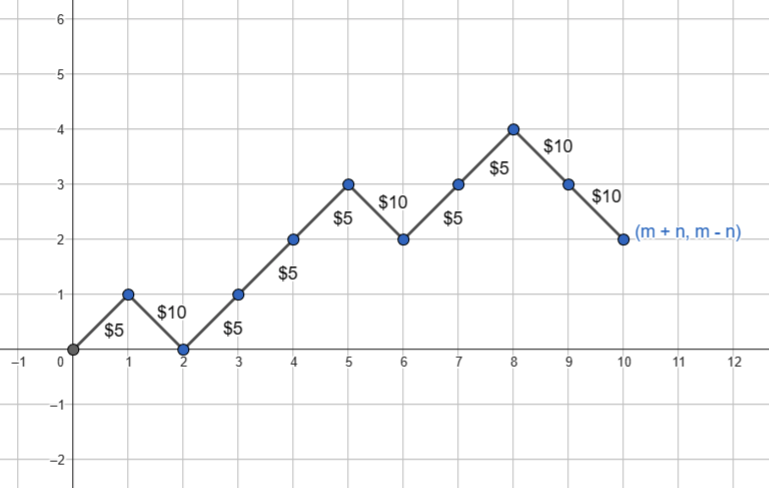
\includegraphics[width=9cm]{26/figs/26_diagram1.png}
\end{center}

The number of such graphs is ${n+m \choose m}$. Notice that a configuration is acceptable, only if we never go below line $y=0$. An example of an unacceptable configuration is given below.

\begin{center}
	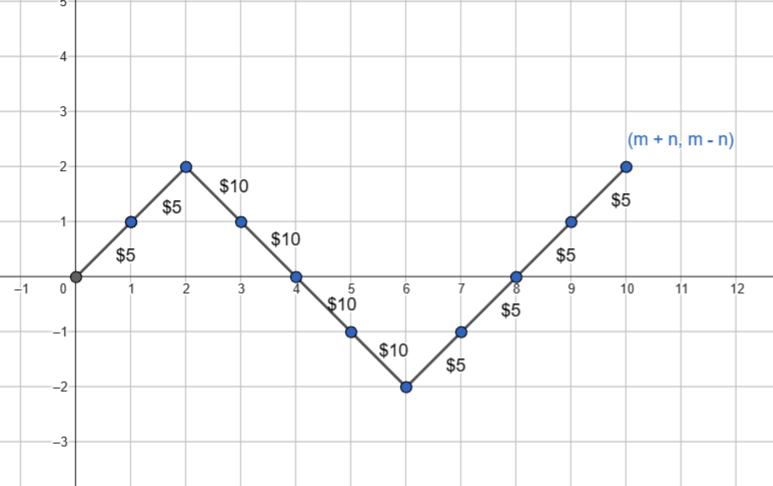
\includegraphics[width=9cm]{26/figs/26_diagram2.png}
\end{center}

To count these unacceptable configurations, we observe that these states are the states where the graph intersects the line y=-1. We show a 1-to-1 mapping between such figures and the ones that start from location $(0,-2)$. To this end, we mirror the graph before the first intersection with line $y=-1$. For example, for the figure above the result would be as follows:

\begin{center}
	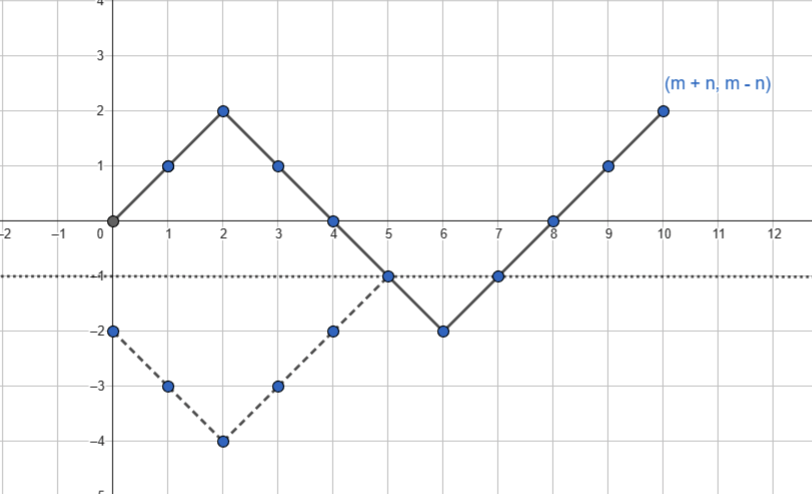
\includegraphics[width=9cm]{26/figs/26_diagram3.png}
\end{center}

Notice that in all such graphs we start from point $(0,-2)$ and end at $(m+n, m-n)$ as before. These diagrams have a one-to-one correspondence with unacceptable states. Thus, the number of such configurations is to ${n+m \choose m+1}$.

So the total number of acceptable configurations is equal to ${n+m \choose m} - {n+m \choose m+1}$. In these configurations, we are indifferent between people who have the same set of bills.
If we also take into account such distinctions, the answer would be the following:

$$
({n+m \choose m} - {n+m \choose m+1}) \times n! \times m!
$$



\end{solution}